\documentclass{beamer}
\usetheme{Rochester}
\usecolortheme{beetle}

\usepackage[shortlabels]{enumitem}
\usepackage{graphicx}
\usepackage{amsmath}
\usepackage{mathtools}
\usepackage[b]{esvect}
\usepackage{tikz}

%Information to be included in the title page:
\title{Project Control}
\subtitle{ECES 512}
\author{Damien Prieur \\ Conor Kennedy}
\date{3/5/2021}

\begin{document}

\frame{\titlepage}

\begin{frame}
\frametitle{Electromechanical Magnetic-Ball Suspension}
\begin{itemize}[$\bullet$]
\item Make an object levitate by controlling the current
\end{itemize}
\begin{figure}
\includegraphics[scale=.75]{"../images/Electromechanical Magnetic-Ball Suspension setup".png}
\end{figure}
\end{frame}

\begin{frame}
\frametitle{Mathematical Model}
Variables
\begin{itemize}
\item $R$ - Resistance
\item $L$ - Inductance
\item $v$ - Voltage
\item $m$ - Mass
\item $K$ - Coefficient that relates force to the magnetic field
\item $g$ - Gravity
\item $i$ - Current
\item $y$ - Distance of Mass M to electromagnet
\end{itemize}
$$
\begin{aligned}
    &\begin{aligned}
        \mathllap{v(t)} &= Ri(t) + L\frac{di(t)}{dt}
    \end{aligned} \\
    &\begin{aligned}
        \mathllap{m\frac{d^2y(t)}{dt^2}} &= mg - K\frac{i^2(t)}{y(t)}
    \end{aligned} \\
\end{aligned}
$$
\end{frame}

\begin{frame}
\frametitle{I/O and State Variables}
\begin{itemize}[$\bullet$]
\item We control the voltage $v$
\item Goal is to control distance $y$
\end{itemize}
$$
\vv{x}=
\begin{bmatrix}
x_1 \\
x_2 \\
x_3
\end{bmatrix}
=
\begin{bmatrix}
i \\
y \\
\dot{y}
\end{bmatrix}
=
\begin{bmatrix}
\text{Current} \\
\text{Distance}\\
\text{Velocity}
\end{bmatrix}
$$

\end{frame}

\begin{frame}
\frametitle{Linearization about the Equilibrium}
$$
\begin{bmatrix}
\dot{x}_1 \\
\dot{x}_2 \\
\dot{x}_3
\end{bmatrix}
=
\begin{bmatrix}
\frac{u(t)-Rx_1(t)}{L} \\
x_3(t) \\
-\frac{Kx_1^2(t)}{mx_2(t)} + g
\end{bmatrix}
$$
$$
A
=
\frac{\partial h}{\partial x}
=
\begin{bmatrix}
-\frac{R}{L} & 0 & 0\\
0 & 0 & 1\\
-\frac{2Kx_1(t)}{mx_2(t)} & \frac{K}{m}(\frac{x_1(t)}{x_2(t)})^2 & 0\\
\end{bmatrix}
=
\begin{bmatrix}
-\frac{R}{L} & 0 & 0\\
0 & 0 & 1\\
-\frac{2Kx_{01}}{mx_{02}} & \frac{K}{m}(\frac{x_{01}}{x_{02}})^2 & 0\\
\end{bmatrix}
$$
$$
B
=
\frac{\partial h}{\partial u}
=
\begin{bmatrix}
\frac{1}{L} \\
0 \\
0 \\
\end{bmatrix}
\qquad
C
=
\begin{bmatrix}
0 & 1 & 0
\end{bmatrix}
\qquad
D
=
\begin{bmatrix}
0
\end{bmatrix}
$$
\\
$$
v_0 = 7 \qquad
x_0
=
\begin{bmatrix}
7 \\
.00998 \\
0
\end{bmatrix}
\qquad
A
=
\begin{bmatrix}
-100 & 0 & 0 \\
0 & 0 & 1 \\
-2.803 & 982 & 0
\end{bmatrix}
$$
\end{frame}

\begin{frame}
\frametitle{Stability}
Internal stability: Look at the eigenvalues of our A matrix
$$
\begin{bmatrix}
-100 & 0 & 0 \\
0 & 0 & 1 \\
-2.803 & 982 & 0
\end{bmatrix}
$$
$$ \lambda_1 = -100 \quad \lambda_2 \approx 31.34 \quad \lambda_3 \approx -31.34 $$
Our system is not internally stable

\end{frame}

\begin{frame}
\frametitle{Stability}
BIBO stability: Look at the transfer function
$$
C ( sI-A ) ^{-1} B
$$
$$
A =
\begin{bmatrix}
-100 & 0 & 0 \\
0 & 0 & 1 \\
-2.803 & 982 & 0
\end{bmatrix}
\qquad B = \begin{bmatrix} 100 \\ 0 \\ 0\end{bmatrix}
\qquad C = \begin{bmatrix} 0 & 1 & 0 \end{bmatrix}
$$
$$ G(s) = \frac{-280}{(s-31.34) (s+31.34) (s+100)} $$
Since we have a pole in the right half plane our system is also not BIBO stable.

\end{frame}

\begin{frame}
\frametitle{Open Loop}
\begin{figure}
\centering
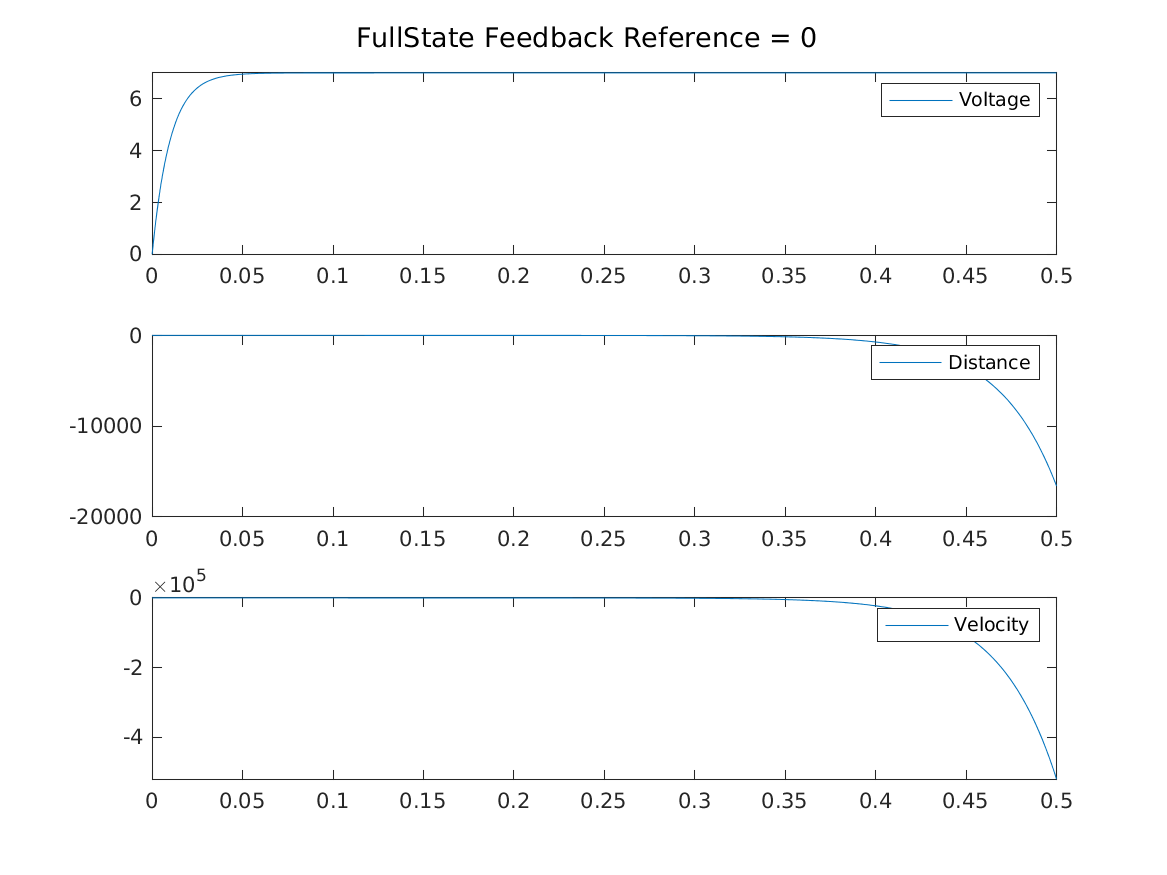
\includegraphics[scale=.5]{{images/OpenLoop_No input}.png}
\end{figure}
\end{frame}

\begin{frame}
\frametitle{Controllability}
Controllability Matrix
$$ \mathcal{C} = \begin{bmatrix} B & AB & A^2B \end{bmatrix} $$
$$
A =
\begin{bmatrix}
-100 & 0 & 0 \\
0 & 0 & 1 \\
-2.803 & 982 & 0
\end{bmatrix}
\qquad B = \begin{bmatrix} 100 \\ 0 \\ 0\end{bmatrix}
$$

$$
\mathcal{C} =
\begin{bmatrix}
100 & -10000 & 10^6 \\
0 & 0 & -280.3 \\
0 & -280.3 & 28030 \\
\end{bmatrix}
$$
$$ \text{rank}(\mathcal{C}) = 3 $$
The system is controllable.
\end{frame}

\begin{frame}
\frametitle{Observability}
Observability Matrix
$$ \mathcal{O} = \begin{bmatrix} C \\ CA \\ CA^2 \end{bmatrix} $$
$$
A =
\begin{bmatrix}
-100 & 0 & 0 \\
0 & 0 & 1 \\
-2.803 & 982 & 0
\end{bmatrix}
\qquad C = \begin{bmatrix} 0 & 1 & 0\end{bmatrix}
$$

$$
\mathcal{O} =
\begin{bmatrix}
0 & 1 & 0 \\
0 & 0 & 1 \\
-2.803 & 982 & 0 \\
\end{bmatrix}
$$
$$ \text{rank}(\mathcal{O}) = 3 $$
The system is Observable.
\end{frame}

\begin{frame}
\frametitle{Desired behavior}
\begin{itemize}[$\bullet$]
\item Can't move too far from linearization range
\item Low to no overshoot (5\% <)
\item Fast response (<.05s)
\end{itemize}
Used bode plot and root locus tools in MATLAB.
\end{frame}

\begin{frame}
\frametitle{Choosing Poles}

\begin{figure}
\centering
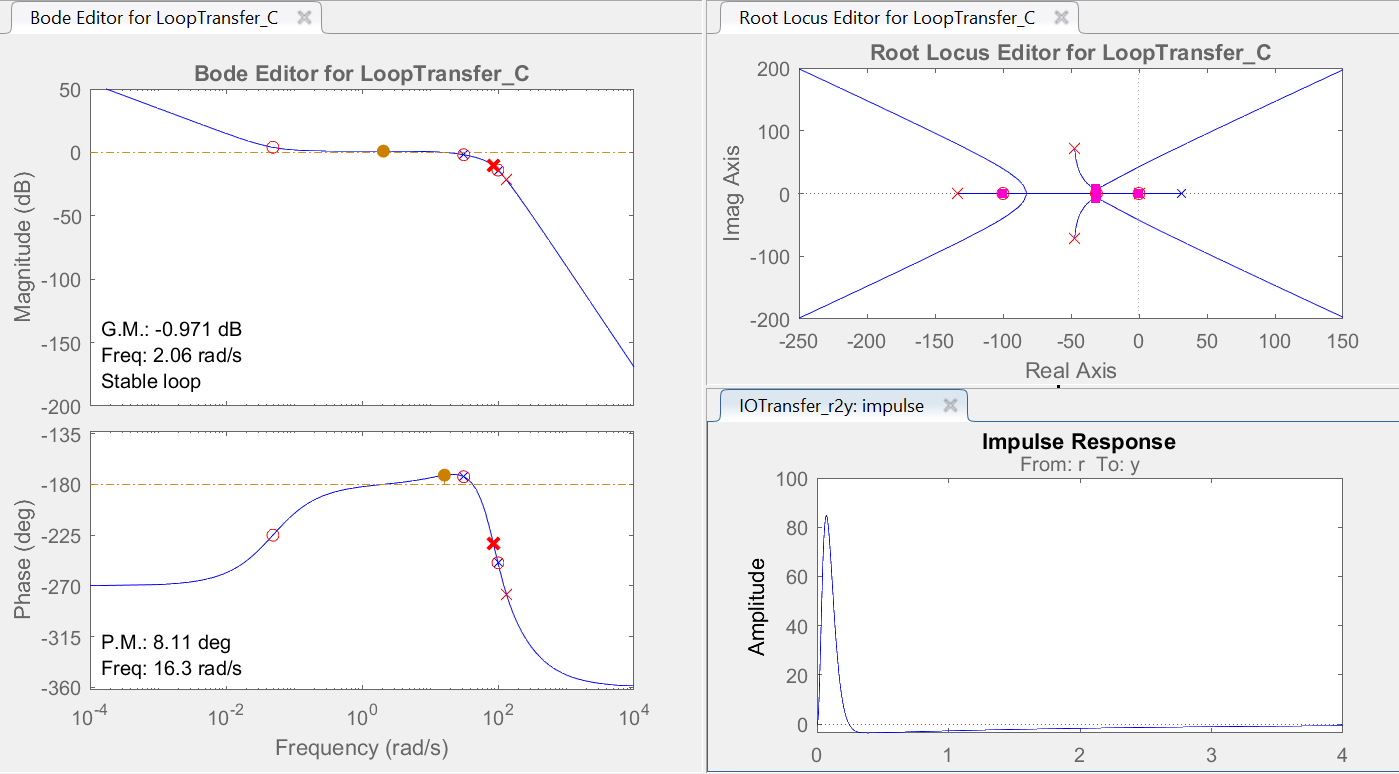
\includegraphics[scale=.19]{{../images/bode_root_locus_plots}.png}
\end{figure}

$$p_1 = -20+20i \qquad p_2 = -20-20i \qquad p_3 = -100 $$
$$ (s-(-20+20i))(s-(-20+20i))(s-(-100)) $$
$$ s^3 + 140s^2 +4800s + 80000 $$
\end{frame}

\begin{frame}
\frametitle{Selecting Gain Matrix}
Using Ackermann's formula we can find the $K$ values to select our desired poles.
$$ k^T = \begin{bmatrix}0 & 0 & 1 \end{bmatrix} \mathcal{C}^{-1} \Delta(A) $$
$$ \Delta(x) = x^3 + 140x^2 + 4800x + 80000 $$
$$ k^T =
\begin{bmatrix}0 & 0 & 1 \end{bmatrix}
\mathcal(C)^{-1}
(A^3 + 140A^2 +4800A + 80000)
$$
$$ k = \begin{bmatrix} -.1 & -458.01 & -13.49 \end{bmatrix} $$
Modified System
$$
\dot{x} =
\begin{bmatrix}
-100 & 0 & 0 \\
0 & 0 & 1 \\
-2.803 & 982 & 0
\end{bmatrix}
x +
\begin{bmatrix} 100 \\ 0 \\ 0\end{bmatrix}
\begin{bmatrix} -.1 & -458.01 & -13.49 \end{bmatrix}
u
$$

\end{frame}

\begin{frame}
\frametitle{Full State Feedback No reference}
\begin{figure}
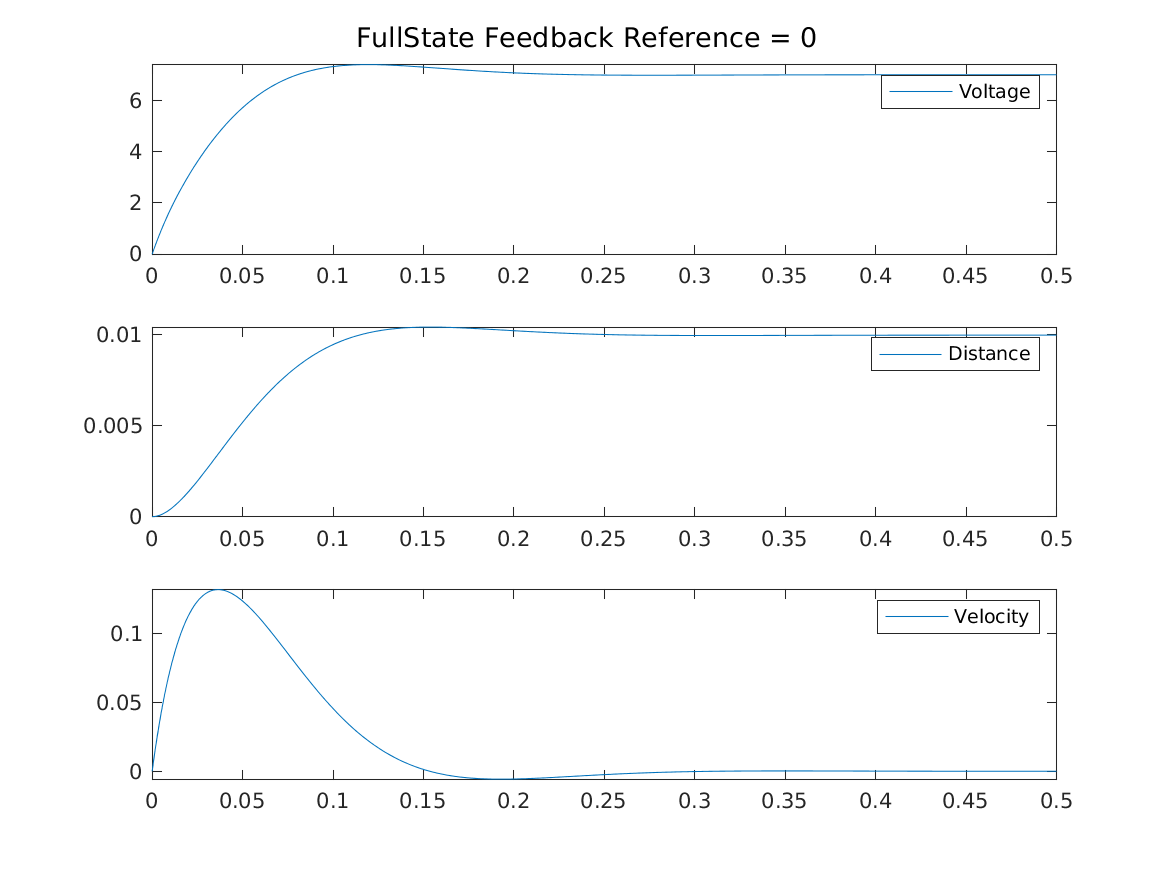
\includegraphics[scale=.5]{images/FullState_Feedback_ref_0.png}
\end{figure}
\end{frame}

\begin{frame}
\frametitle{Full State Feedback without $\bar{N}$}
\begin{figure}
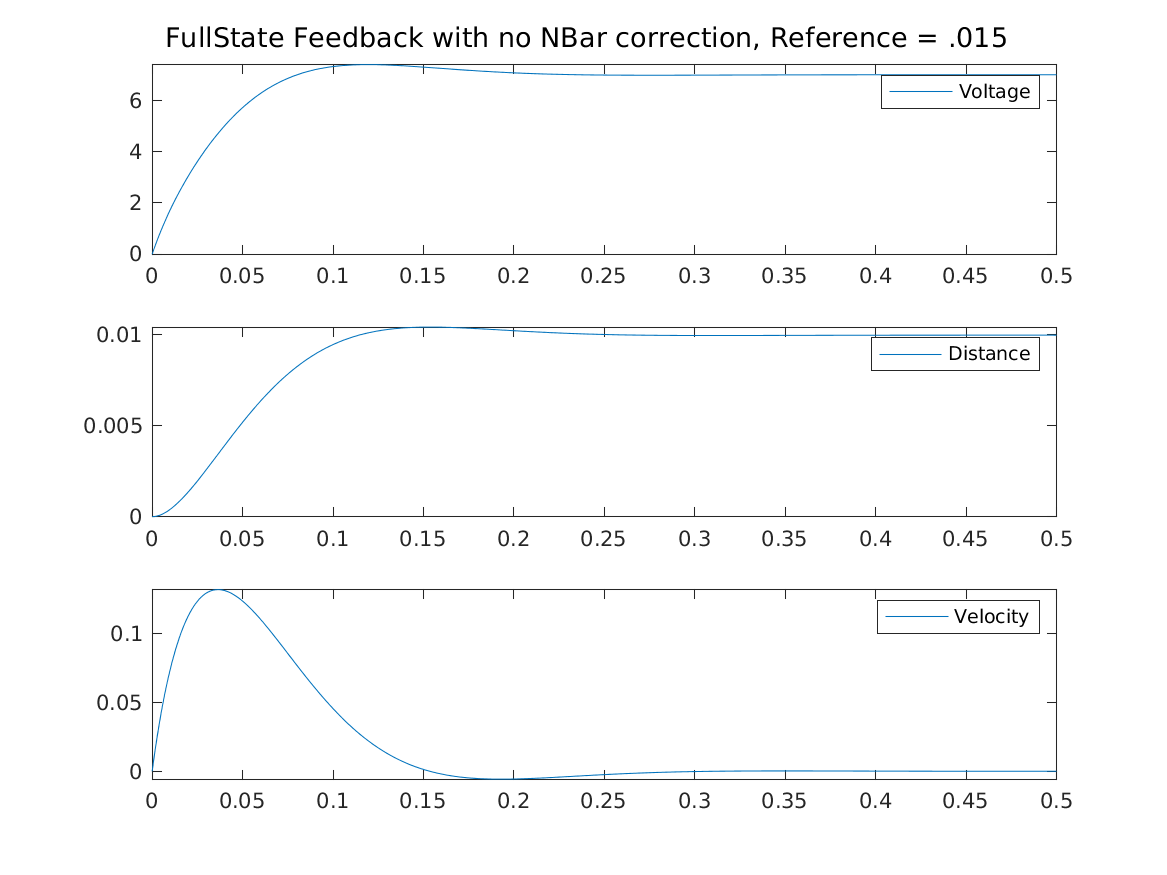
\includegraphics[scale=.5]{images/FullState_Feedback_No_nBar_ref_p015.png}
\end{figure}
\end{frame}

\begin{frame}
\frametitle{Choosing $\bar{N}$}
$$\bar{N}\frac{Y(S)}{R(S)}_{s->0} = 1 $$
$$ \bar{N} = \frac{R(S)}{Y(S)}_{s->0} $$
$$ \frac{Y(s)}{R(s)} = C(sI - (A-BK))^{-1}B = -\frac{280.3}{s^3+140s^2+4800s+80000} $$
Evaluating at $s->0$ we get $ \frac{-280.3}{80000} $
Solving for $\bar{N}$ we get
$$ \bar{N} = \frac{-80000}{280} \approx -285.72 $$
\end{frame}

\begin{frame}
\frametitle{Full State Feedback with $\bar{N}$}
\begin{figure}
\centering
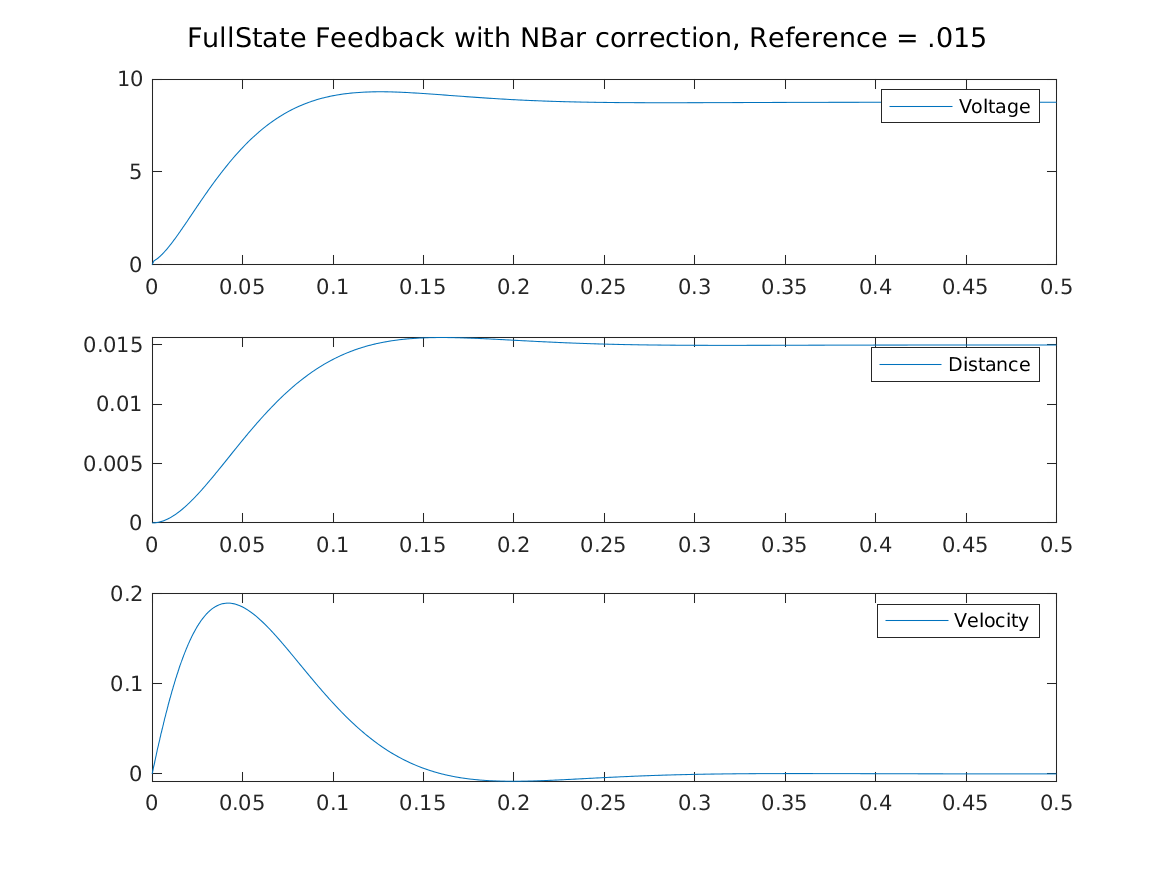
\includegraphics[scale=.5]{images/FullState_Feedback_with_nBar_ref_p015.png}
\end{figure}
\end{frame}

\begin{frame}
\frametitle{Observer Gain Matrix}
Choose our poles to be 5 times further than the poles of the control matrix.
$$p_1 = -100+100i \qquad p_2 = -100-100i \qquad p_3 = -500 $$
$$ (s-(-100+100i))(s-(-100+100i))(s-(-500)) $$
$$ s^3 + 700*s^2 + 120000*s + 10000000 $$
Using Ackermann's formula we can find the $L$ values to select our desired poles.
$$ l^T = \Delta(A) \mathcal{O}^{-1} \begin{bmatrix}0 \\ 0 \\ 1 \end{bmatrix} $$
$$ \Delta(x) = x^3 + 90x^2 +2800x + 40000 $$
$$ l = \begin{bmatrix} -1.427 \times 10^6 \\ 600 \\ 60892 \end{bmatrix} $$
\end{frame}

\begin{frame}
\frametitle{Output Feedback System}
$$
\begin{bmatrix}
\dot{x} \\
\dot{\hat{x}} \\
\end{bmatrix}
=
\begin{bmatrix}
A & -Bk \\
lC & A-Bk-lC \\
\end{bmatrix}
\begin{bmatrix}
x \\
\hat{x} \\
\end{bmatrix}
+
\begin{bmatrix}
B \\
B \\
\end{bmatrix}
u
$$
$$
\begin{bmatrix}
y \\
\hat{y} \\
\end{bmatrix}
=
\begin{bmatrix}
C & 0 \\
0 & C \\
\end{bmatrix}
\begin{bmatrix}
x \\
\hat{x} \\
\end{bmatrix}
+
0
$$
\end{frame}

\begin{frame}
\frametitle{Output Feedback no Reference}
\begin{figure}
\centering
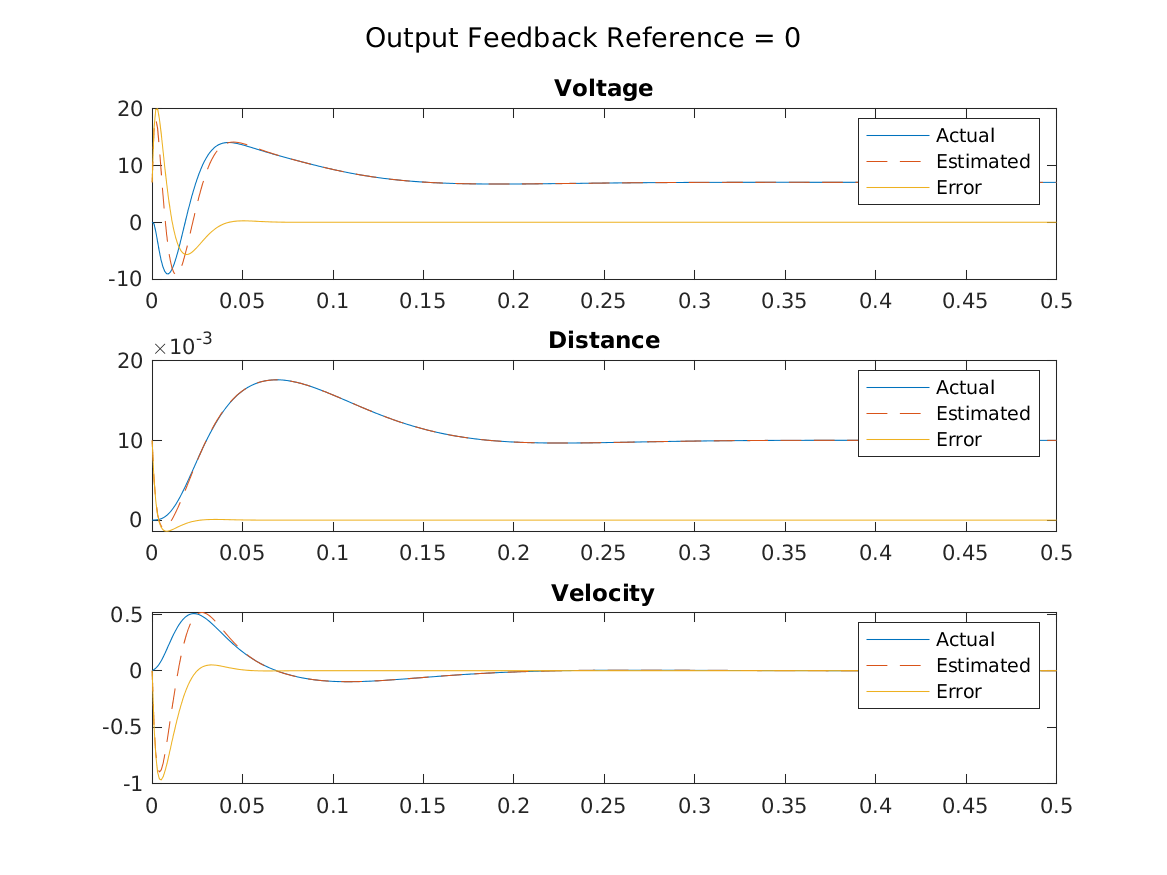
\includegraphics[scale=.5]{images/Output_Feedback_ref_0.png}
\end{figure}
\end{frame}

\begin{frame}
\frametitle{Output Feedback with Reference}
\begin{figure}
\centering
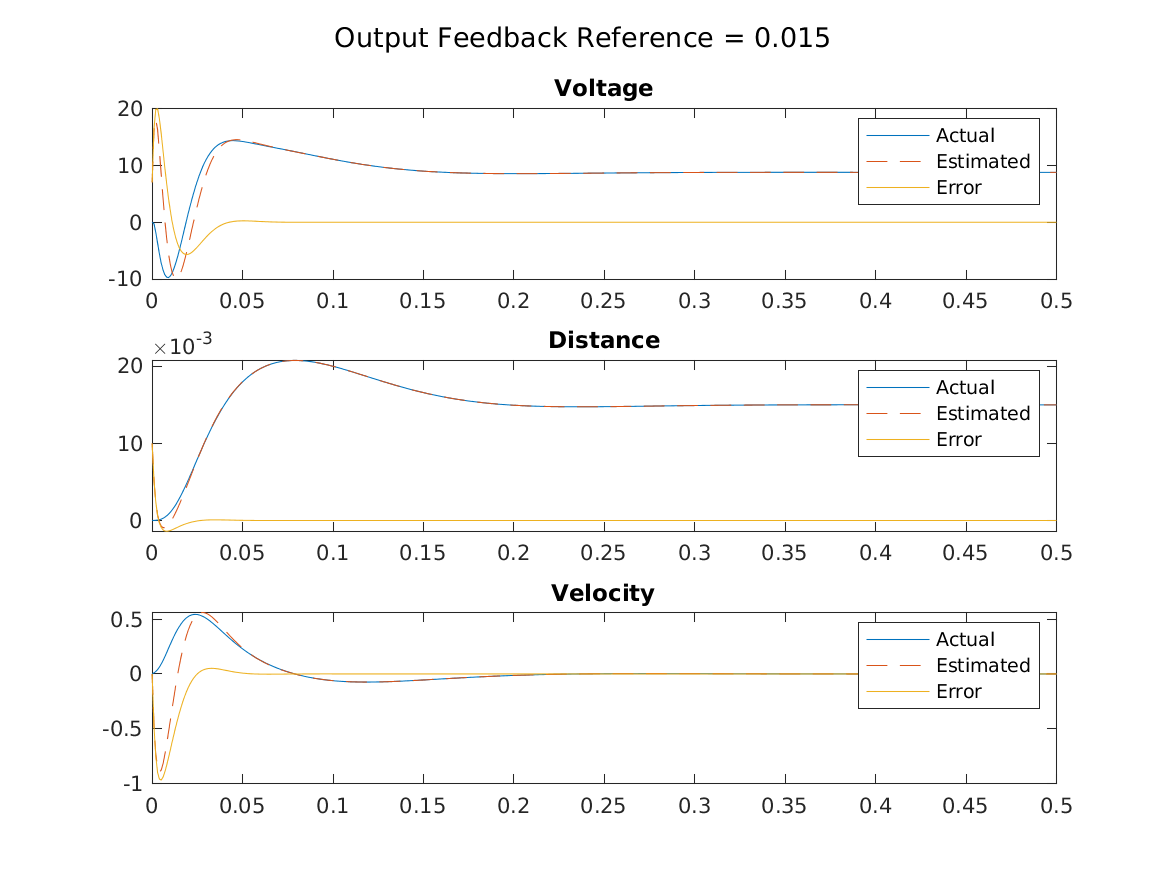
\includegraphics[scale=.5]{images/Output_Feedback_ref_p015.png}
\end{figure}
\end{frame}

\begin{frame}
\frametitle{References}
\begin{enumerate}[1.]
\item \url{http://ctms.engin.umich.edu/CTMS/index.php?example=Introduction\&section=ControlStateSpace}
\item \url{https://elec3004.uqcloud.net/laboratories/LeviLab/Levitating\%20Magnet\%20Modelling\%20Example.pdf}
\end{enumerate}
\end{frame}


\end{document}
